\section{Durchführung}
\label{sec:Durchführung}
Der Versuchsablauf lässt sich in Fourier-Analyse und Fourier-Synthese unterteilen.

\subsection{Vorbereitung}
Vor Beginn der Messreihe werden die Fourier-Koeffizienten der ausgewählten Rechteck-,
Dreieck-, und Sägezahnspannung (beispielhaft dargestellt in Abbildung 2 bis 4) bestimmt. Dazu werden diese zur Vereinfachung so parametrisiert,
dass es sich um gerade bzw. ungerade Funktionen handelt, da so $b_\text{n} = 0$ bzw.
$a_\text{n} = 0$ gilt. Die berechneten Koeffizienten lauten:

%Rechteck
\begin{figure}[H]
\hspace{73pt}
\begin{minipage}[t]{6cm}
\vspace{0pt}
\centering
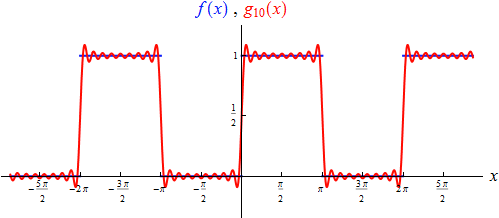
\includegraphics[scale=0.5]{vorb1.png}
\caption{Eine Rechteckspannung und die zugehörige Fourierreihe \cite{sample2}.}
\label{fig:vorb1}
\end{minipage}
\hfill
\hspace{73pt}
\begin{minipage}[t]{6cm}
\vspace{0pt}
Rechteckspannung: \\
$a_\text{n} = 0$, \\
$b_\text{n gerade} = 0$, \\
$b_\text{n ungerade} = \frac{4}{\pi n}$,
\end{minipage}
\end{figure}


%Dreieck
\begin{figure}[H]
\hspace{73pt}
\begin{minipage}[t]{6cm}
\vspace{0pt}
\centering
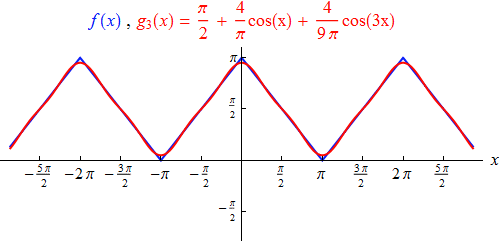
\includegraphics[scale=0.5]{vorb2.png}
\caption{Eine Dreieckspannung und die zugehörige Fourierreihe \cite{sample2}.}
\label{fig:vorb2}
\end{minipage}
\hfill
\hspace{73pt}
\begin{minipage}[t]{6cm}
\vspace{0pt}
Dreieckspannung: \\
$a_\text{n gerade} = 0$, \\
$a_\text{n ungerade} = - \frac{4}{\pi n^{2}}$, \\
$b_\text{n} = 0$,
\end{minipage}
\end{figure}

%Sägezahn
\begin{figure}[H]
\hspace{73pt}
\begin{minipage}[t]{6cm}
\vspace{0pt}
\centering
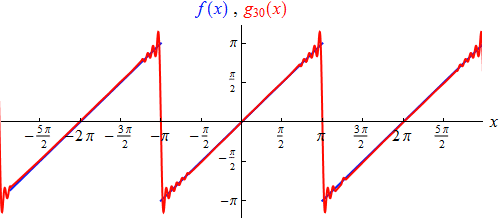
\includegraphics[scale=0.5]{vorb3.png}
\caption{Eine Sägezahnspannung und die zugehörige Fourierreihe \cite{sample2}.}
\label{fig:vorb3}
\end{minipage}
\hfill
\hspace{73pt}
\begin{minipage}[t]{6cm}
\vspace{0pt}
Sägezahnspannung: \\
$a_\text{n} = 0$, \\
$b_\text{n gerade} = - \frac{2}{n}$, \\
$b_\text{n ungerade} = \frac{2}{n}$.
\end{minipage}
\end{figure}

\subsection{Fourier-Analyse}
Für die Fourier-Analyse wird ein Funktionsgenerator an ein digitales Oszilloskop angeschlossen.
Das Oszilloskop führt die Fourier-Transformation des Signals durch und stellt diese dar.
Die Amplituden der Maxima dieser Transformation werden über die Cursor-Funktion gemessen
und notiert, wobei Nebenmaxima ignoriert werden.

\subsection{Fourier-Synthese}
Zunächst werden nacheinander zwei Ausgänge eines Oberwellengenerators an das Oszilloskop angeschlossen.
Nur eins der Kabel wandert hierbei durch alle möglichen Ausgänge $A_\text{2-9}$ des Oberwellengenerators, das andere bleibt
im Ausgang $A_\text{1}$. Das Oszilloskop wird nun in den X-Y-Betrieb geschaltet, mit dem Ziel,
alle Ausgänge des Generators in Phase zu schalten. Hierzu wird die Amplitude zunächst maximal eingestellt,
da so die höchste Genauigkeit erlangt werden kann. Die Phasen der einzelnen Generatoren werden
nun solange justiert bis sich auf dem Oszilloskopen Lissajous-Figuren ausbilden.

Im Folgenden werden die Amplituden der Generatoren mithilfe der in der Vorbereitung errechneten
Proportionalitätsfaktoren so eingestellt, dass durch eine Überlagerung aller Einzelschwingungen
die gewünschte zusammengesetzte Schwingung entsteht. Dazu werden alle Ausgänge nacheinander
an ein Voltmeter angeschlossen. Das Oszilloskop wird nach dem Einstellen der Amplituden
 zurück in den X-T-Betrieb geschaltet. Es wird der summierte Ausgang des 
Oberwellengenerators mit dem Oszilloskop verbunden, sodass die Überlagerung aller Schwingungen
auf dem Oszilloskop dargestellt wird. Gegebenenfalls werden einige Oberwellen um 180° in der
Phase verschoben, wenn so die Approximation der zu synthetisierenden Spannung besser gelingt.

Im Fall der Sägezahn- und der Rechteckspannungsynthese beträgt dieser Proportionalitätsfaktor 
$\frac{1}{n}$. Für die Dreieckspannung beträgt er $\frac{1}{n^{2}}$.

Zuletzt wird ein Abbild der synthetisierten Spannungen erstellt.